\section{Results}\label{sec:results}
This sections presents the constraint on $\fnl$ from the DR9 LRG sample. We also validate the modeling pipeline and characterize the amount of mitigation bias introduced in $\fnl$ after cleaning for systematics. 



\subsection{DR9 LRGs}
Fig. \ref{fig:cl_dr9} shows the measured power spectrum of DR9 LRGs with different imaging weights, the best fit theory curves, and the mean and 1$\sigma$ error from the $\fnl=0$ lognormal mocks. Power spectra are similar with differences less than ??\% for small scales ($\ell > 2$), and as we go to larger scales, the differences become more significant. There is a little difference between linear cons II and linear all maps. This proves that our feature selection procedure has worked to identify the important maps. Comparing linear cons I to linear cons II, modes with $6\leq \ell < 10$ are different, indicating scales where psfsize-r is affecting the signal. Comparing nonlinear cons II to linear cons II, modes at the second bin ($4 \leq \ell < 6$) are very different, indicating the nonlinear approach is more flexible to reduce fluctuations on small scales as well large scales. 

\begin{figure}
    \centering
    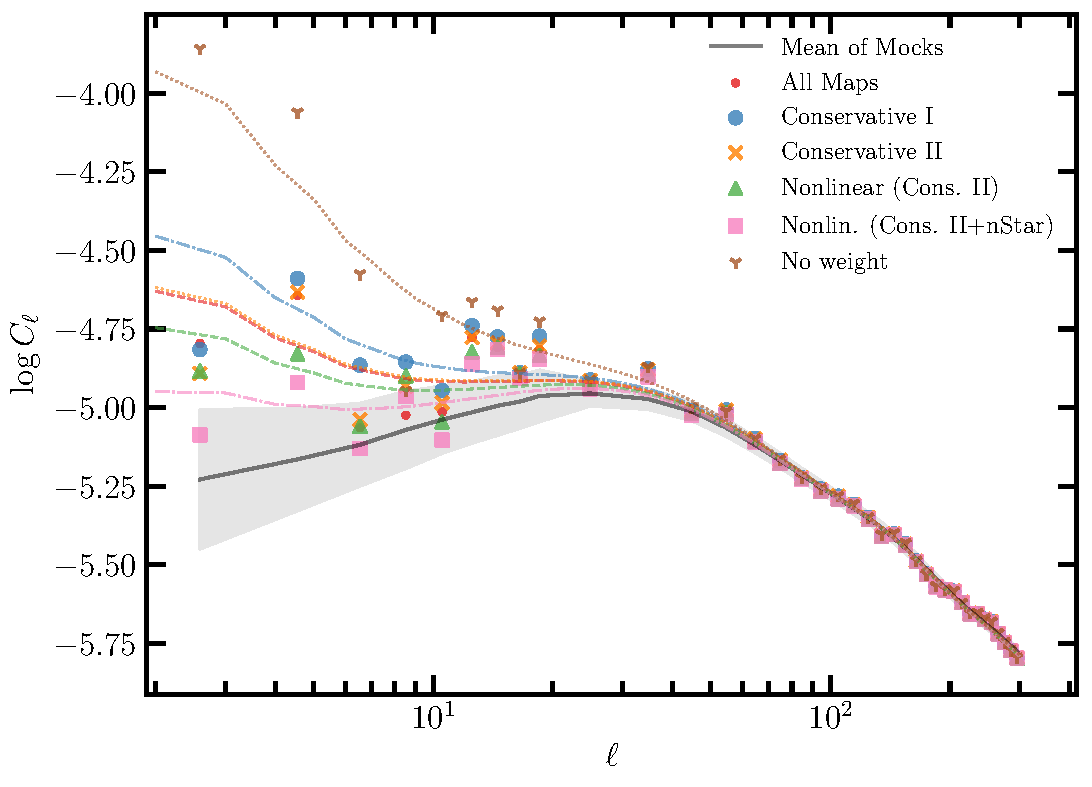
\includegraphics[width=0.45\textwidth]{figures/model_dr9.pdf} 
    \caption{Measured power spectrum of the DR9 LRG sample before and after correcting for systematics with their corresponding best fit theory predictions. The shade represents $1\sigma$ error constructed from the $\fnl=0$ mocks.}
    \label{fig:cl_dr9}
\end{figure}


$\fnl$ constraints from DR9 LRG sample is summarized in Table \ref{tab:dr9method}. First, we focus on the DESI footprint and then compare constraints obtained from each sub-survey. Before correction, we obtain $98.14<\fnl<132.89$ with a best fit of $113.18$ and marginalized mean of $115.49$. Applying imaging weights shifts constraints to lower $\fnl$ values. Using all maps with the linear model does not change the results, showing that three maps are sufficient.  However, using a nonlinear model instead shows around $1\sigma$ shift. Adding a template for the local stellar density shift constraints by $1\sigma$ and using all maps results in more than $2\sigma$ shift. We emphasize that however these shifts are somewhat expected as inputing more maps results in regressing more of cosmological clustering signal. Therefore, we use lognormal mocks to calibrate the amount of signal that is removed in each case and attempt to undo the effect.


Now we evaluate the robustness of constraints against various cuts and configurations.

\textbf{Pixel completeness}
We remove pixels with low completeness from the mask by applying $f_{\rm pix}>0.5$. At the cost of losing $.6\%$ survey area, we find that the $\fnl$ constraint changes only around $2\%$, from 28.58 to 28.07, see \textit{comp cut} Table \ref{tab:dr9method}.


\textbf{Imaging quality}
We remove pixels with poor imaging from the mask by applying the following limits on imaging properties; $E[B-V]<0.1$, $nStar < 3000$, $depth_{g} > 23.2$, $depth_{r} > 22.6$, $depth_{z} > 22.5$, $psfsize_{g}<2.5$, $psfsize_{r}<2.5$, and $psfsize_{z}<2$. We lose about $8.2\%$ survey area, and the best fit $\fnl$ estimate changes about $2\%$ from $28.58$ to $29.16$. See \textit{imag cut} in Table \ref{tab:dr9method}.


\textbf{Covariance}
The mocks with $\fnl=76.92$ are used to construct a covariance matrix, and with the new covariance we obtain a $12\%$ increase in the $\fnl$ constraint uncertainties and $11\%$ change in the best fit.

\begin{table*}
    \caption{Maximum-A-Posteriori (MAP) and marginalized mean estimates for $\fnl$ from fitting power spectrum of DR9 LRGs before and after correcting for systematics. Degree of freedom is 34 (37 data points - 3 parameters).}
    \label{tab:dr9method}
   \centerline{%     
    \begin{tabular}{llllllll}
    \hline
    \hline
   &  & 	  & & $\fnl$ &  &  \\
   \cmidrule(r{.7cm}){3-6}
Footprint   & Method & 	Best fit  & Mean & $ 68\%$ CL & $ 95\%$ CL & $\chi^{2}$ \\
    \hline
DESI                      & No Weight   & $113.18$& $115.49$& $ 98.14<\fnl<132.89$& $ 83.51<\fnl<151.59$ &   44.4\\
DESI                      & Linear (All Maps)& $ 36.05$& $ 37.72$& $ 26.13<\fnl< 49.21$& $ 16.31<\fnl< 62.31$ &   41.1\\
DESI                      & Linear (Conservative I)& $ 49.58$& $ 51.30$& $ 38.21<\fnl< 64.33$& $ 27.41<\fnl< 78.91$ &   38.8\\
DESI                      & Linear (Conservative II)& $ 36.63$& $ 38.11$& $ 26.32<\fnl< 49.86$& $ 16.36<\fnl< 63.12$ &   39.6\\
DESI                      & Nonlinear (Cons. II)& $ 28.58$& $ 29.79$& $ 18.91<\fnl< 40.59$& $  9.47<\fnl< 52.73$ &   34.6\\
DESI                      & Nonlin. (Cons. II+nStar)& $ 16.63$& $ 17.52$& $  7.51<\fnl< 27.53$& $ -1.59<\fnl< 38.49$ &   35.2\\
DESI                      & Nonlin. (All Maps+nStar)& $ -5.87$& $ -9.19$& $-21.45<\fnl<  2.40$& $-33.81<\fnl< 12.06$ &   39.5\\
DESI (imag. cut)          & Nonlin. (Cons. II)& $ 29.16$& $ 30.57$& $ 19.05<\fnl< 42.18$& $  9.01<\fnl< 54.81$ &   35.8\\
DESI (comp. cut)          & Nonlin. (Cons. II)& $ 28.07$& $ 29.48$& $ 18.38<\fnl< 40.50$& $  8.81<\fnl< 53.10$ &   34.5\\
DESI                      & Nonlin. (Cons. II)+$f_{\rm NL}=76.92$ Cov& $ 31.62$& $ 33.11$& $ 20.94<\fnl< 45.24$& $ 10.56<\fnl< 59.16$ &   33.5\\
\hline
BASS+MzLS                 & Nonlin. (Cons. II)& $ 15.43$& $ 19.01$& $ -1.17<\fnl< 39.43$& $-19.19<\fnl< 63.56$ &   35.6\\
BASS+MzLS                 & Nonlin. (Cons. II+nStar)& $ 13.12$& $ 15.39$& $ -4.59<\fnl< 35.56$& $-24.88<\fnl< 59.31$ &   34.7\\
BASS+MzLS                 & Nonlin. (All Maps+nStar)& $ -3.73$& $ -6.34$& $-27.11<\fnl< 13.75$& $-47.44<\fnl< 33.94$ &   36.8\\
BASS+MzLS (imag. cut)     & Nonlin. (Cons. II)& $ 25.03$& $ 29.12$& $  6.16<\fnl< 52.44$& $-14.22<\fnl< 80.54$ &   36.2\\
BASS+MzLS (comp. cut)     & Nonlin. (Cons. II)& $ 16.99$& $ 20.90$& $  0.26<\fnl< 41.76$& $-18.30<\fnl< 67.12$ &   35.8\\
DECaLS North              & Nonlin. (Cons. II)& $ 41.02$& $ 44.89$& $ 23.33<\fnl< 66.78$& $  4.96<\fnl< 93.02$ &   41.1\\
DECaLS North              & Nonlin. (Cons. II+CALIBZ+HI)& $ 55.46$& $ 60.44$& $ 36.78<\fnl< 84.05$& $ 17.86<\fnl<112.81$ &   38.4\\
DECaLS North              & Nonlin. (Cons. II+nStar)& $ 31.45$& $ 34.78$& $ 14.14<\fnl< 55.79$& $ -5.81<\fnl< 80.80$ &   41.2\\
DECaLS North              & Nonlin. (All Maps+nStar)& $  0.81$& $ -5.68$& $-29.73<\fnl< 16.71$& $-53.15<\fnl< 36.19$ &   45.1\\
DECaLS North + islands & Nonlin. (Cons. II)& $ 41.05$& $ 44.82$& $ 23.58<\fnl< 66.08$& $  6.40<\fnl< 91.42$ &   40.7\\
DECaLS North (imag. cut)  & Nonlin. (Cons. II)& $ 43.27$& $ 48.39$& $ 24.60<\fnl< 72.50$& $  4.71<\fnl<101.42$ &   35.1\\
DECaLS North (comp. cut)  & Nonlin. (Cons. II)& $ 40.55$& $ 44.63$& $ 22.41<\fnl< 67.11$& $  3.95<\fnl< 94.06$ &   41.4\\
DECaLS South              & Nonlin. (Cons. II)& $ 31.24$& $ 33.21$& $ 14.89<\fnl< 52.40$& $ -5.11<\fnl< 74.35$ &   30.2\\
DECaLS South              & Nonlin. (Cons. II+CALIBZ+HI)& $ 33.79$& $ 37.50$& $ 17.71<\fnl< 57.42$& $ -0.31<\fnl< 80.94$ &   30.8\\
DECaLS South              & Nonlin. (Cons. II+nStar)& $ 14.34$& $  6.28$& $-21.19<\fnl< 30.01$& $-53.63<\fnl< 49.51$ &   31.9\\
DECaLS South              & Nonlin. (All Maps+nStar)& $-36.76$& $-32.01$& $-49.38<\fnl<-13.61$& $-65.26<\fnl<  7.52$ &   31.5\\
DECaLS South + DEC < $-30$ & Nonlin. (Cons. II)& $ 43.79$& $ 46.79$& $ 30.16<\fnl< 63.41$& $ 16.38<\fnl< 82.72$ &   23.8\\
DECaLS South (imag. cut)  & Nonlin. (Cons. II)& $ 26.47$& $ 23.36$& $  3.18<\fnl< 47.84$& $-57.69<\fnl< 71.39$ &   30.0\\
DECaLS South (comp. cut)  & Nonlin. (Cons. II)& $ 29.62$& $ 31.76$& $ 13.00<\fnl< 51.58$& $ -9.78<\fnl< 74.28$ &   29.7\\
   \hline
    \end{tabular}
}
\end{table*}

%\begin{figure}
%\centering
%    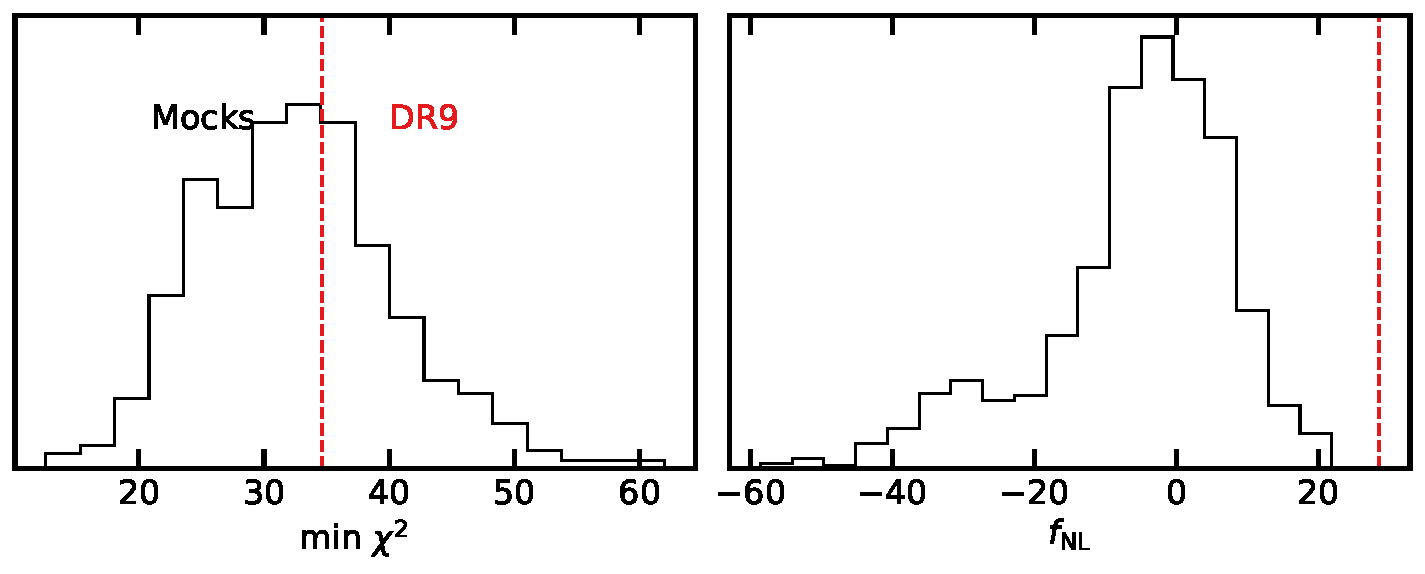
\includegraphics[width=0.45\textwidth]{figures/pdf_dr9vsmocks.pdf} 
%    \caption{Best fit $\chi^{2}$ and $\fnl$ from fitting mocks (histograms) and DR9 (vertical line).}\label{fig:dr9vsmocks}
%\end{figure}

\begin{figure}
    \centering
    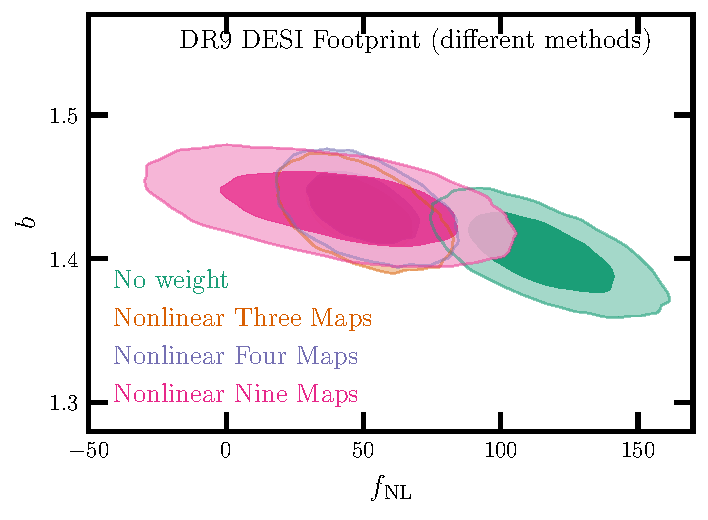
\includegraphics[width=0.45\textwidth]{figures/mcmc_dr9methods.pdf} 
    \caption{DR9 constraints. DESI footprint before and after applying various cleaning methods.}\label{fig:mcmc_dr9}
\end{figure}

\begin{figure}
    \centering
    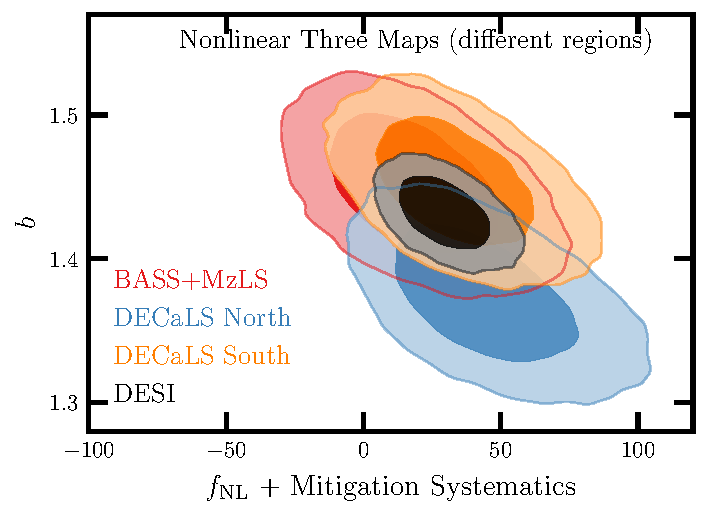
\includegraphics[width=0.45\textwidth]{figures/mcmc_dr9regions.pdf} 
    \caption{DR9 constraints. Each individual imaging survey versus the whole DESI footprint.}\label{fig:mcmc_dr9reg}
\end{figure}

\begin{figure}
    \centering
    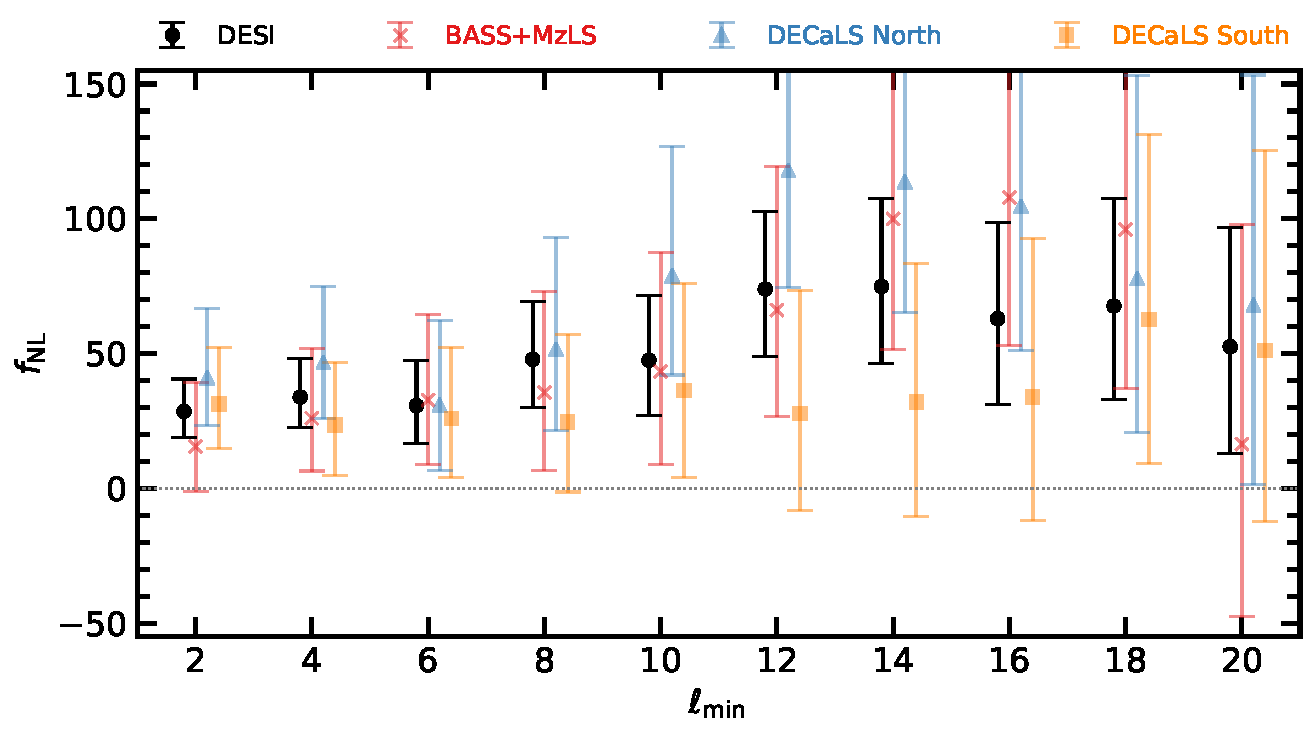
\includegraphics[width=0.45\textwidth]{figures/fnl_elmin.pdf}     
    \caption{DR9 Constraints. Mean estimates of $\fnl$ and its $65$\% and $95$\% errorbars after changing the lowest $\ell$ mode used in fitting.}\label{fig:mcmc_dr9elmin}
\end{figure}


\subsection{Lognormal Mocks}
Corner plots of the PNG parameter $\fnl$ and bias coefficient are shown in Fig. \ref{fig:mcmc_mocks} for fitting the mean power spectrum of the mocks, with and without $\fnl$. Maximum-A-Posteriori estimates and marginalized mean, median and $1\sigma$ quantiles are summarized in Tab. \ref{tab:mocksmcmc}. Comparing DECaLS North with sky coverage $0.14$ to full DESI with $0.40$, we find the constraint improve by a factor of $1.9$ which is slightly more than $\sim f_{\rm SKY}^{-1/2}$, 1.7. while As a robustness test, we also fit the mean power spectrum of the $\fnl=100$ mocks using the covariance matrix estimated from the $\fnl=0$ mocks. We find that the constraints improve by a factor of $4.2$, due to a higher signal to noise ratio.

\begin{table*}
  %\begin{center}
    \caption{Maximum-A-Posteriori (MAP) and marginalized mean estimates for $\fnl$ from fitting the mean power spectrum of the mocks. Degree of freedom is 34 (37 data points - 3 parameters).}   
    \label{tab:mocksmcmc}  
   \centerline{%
    \begin{tabular}{clllllll}
    \hline
    \hline
   &  & 	  & & & $\fnl$ &  \\
   \cmidrule(r{.7cm}){4-7}    
True $\fnl$ &  Footprint   &  Observable & 	Best fit  & Mean & $ 68\%$ CL & $ 95\%$ CL & $\chi^{2}$ \\
    \hline
$76.92$ & DESI & log$C_{\ell}$           & $ 77.67$& $ 77.67$& $ 77.17<\fnl< 78.16$& $ 76.71<\fnl< 78.64$ &   38.8\\
$76.92$ & DESI & $C_{\ell}$              & $ 77.67$& $ 77.65$& $ 77.17<\fnl< 78.14$& $ 76.70<\fnl< 78.60$ &   39.0\\
$76.92$ & DESI & log$C_{\ell}$ + $f_{\rm NL}=0$ cov & $ 77.70$& $ 77.71$& $ 77.25<\fnl< 78.17$& $ 76.81<\fnl< 78.63$ &   39.9\\
$76.92$ & DESI & $C_{\ell}$ + $f_{\rm NL}=0$ cov & $ 77.03$& $ 77.02$& $ 76.93<\fnl< 77.12$& $ 76.83<\fnl< 77.22$ &  207.6\\
\hline
$0$ & DESI         &  log$C_{\ell}$     & $  0.36$& $  0.36$& $  0.06<\fnl<  0.65$& $ -0.23<\fnl<  0.94$ &   35.7\\
$0$ & DECaLS North &  log$C_{\ell}$     & $  0.07$& $  0.06$& $ -0.47<\fnl<  0.60$& $ -1.00<\fnl<  1.12$ &   26.7\\
$0$ & DECaLS South &  log$C_{\ell}$     & $  0.67$& $  0.67$& $  0.13<\fnl<  1.22$& $ -0.40<\fnl<  1.75$ &   34.3\\
$0$ & BASS+MzLS    &  log$C_{\ell}$     & $  0.83$& $  0.82$& $  0.25<\fnl<  1.40$& $ -0.31<\fnl<  1.96$ &   39.4\\
\hline
    \end{tabular}
    }
\end{table*}


\begin{figure*}
    \centering
    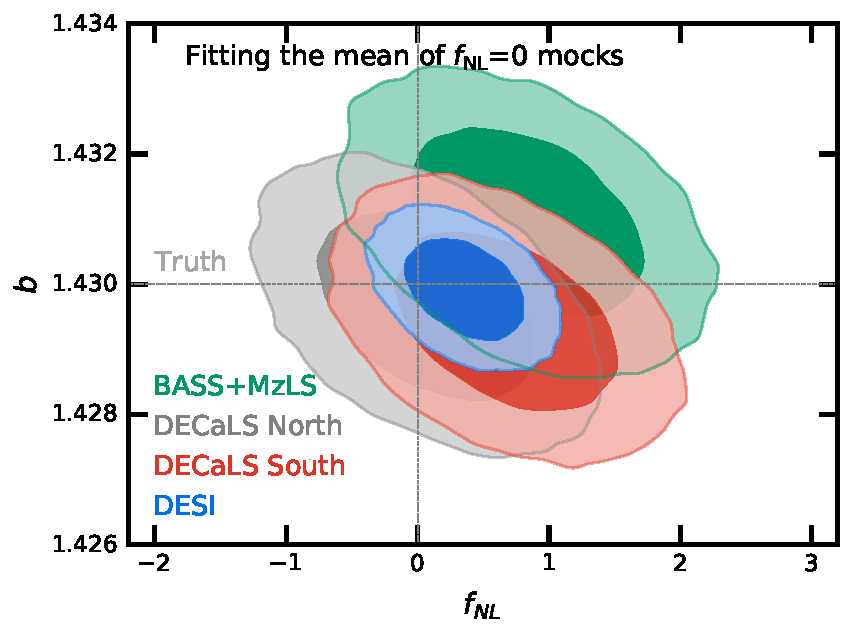
\includegraphics[width=0.45\textwidth]{figures/mcmc_zero.pdf} 
    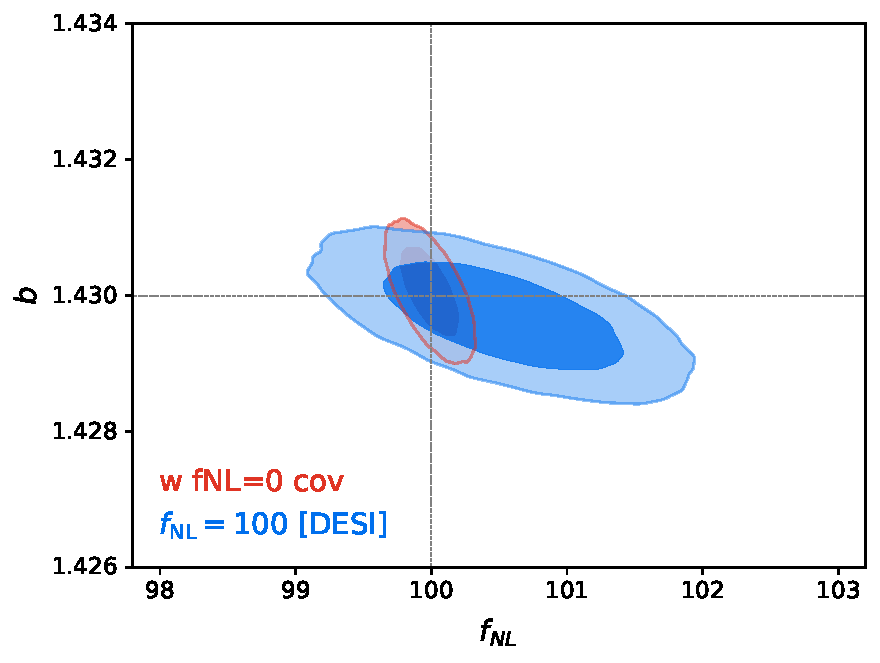
\includegraphics[width=0.45\textwidth]{figures/mcmc_po100.pdf} 
    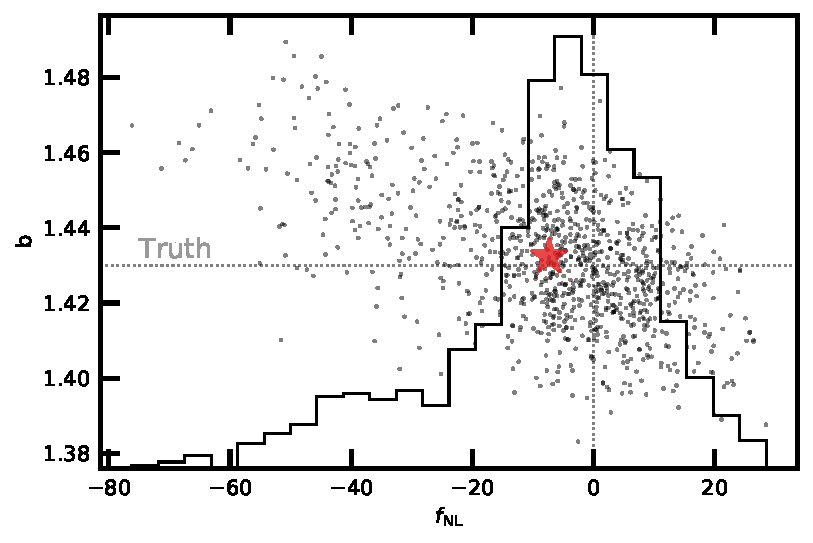
\includegraphics[width=0.45\textwidth]{figures/bestfit_zero.pdf} 
    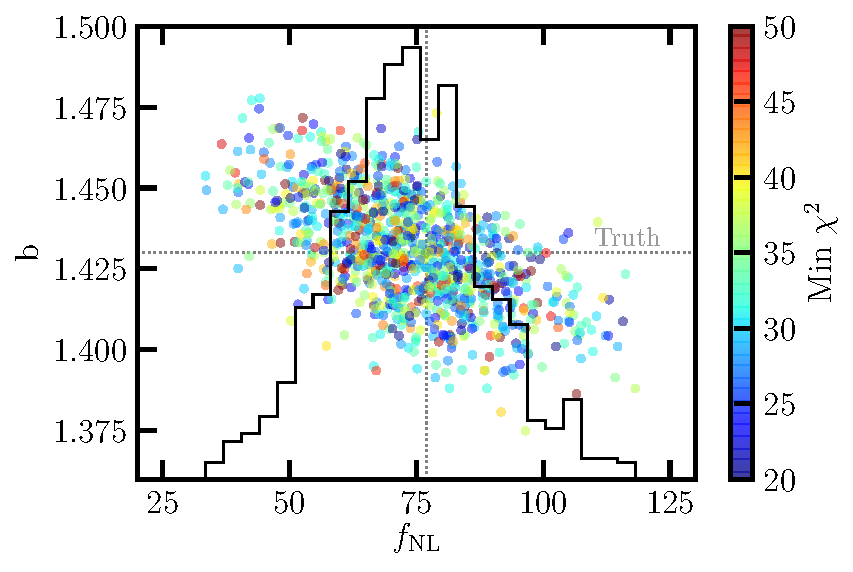
\includegraphics[width=0.45\textwidth]{figures/bestfit_po100.pdf}         
    \caption{Top: 68\% and 95\% confidence contours for $\fnl=0$ (left) and $100$ (right) mocks. Using the $\log C_{\ell}$ fitting yield constraints that are insensitive to the covariance used. Bottom: best fit estimates from fitting 1000 lognormal mocks with $\fnl=0$ (left) and $76.92$ (right) in the DESI footprint. The truth values are represented by vertical and horizontal lines.}\label{fig:mcmc_mocks}
\end{figure*}





\begin{table*}
  %\begin{center}
    \caption{Best fit and marginalized estimates for $\fnl$ from fitting the mean power spectrum of the mocks before and after applying imaging weights. }   
    \label{tab:contmocksmcmc}  
   \centerline{%
    \begin{tabular}{cllllll}
    \hline
    \hline
   &  & 	  & & & $\fnl$ &  \\
   \cmidrule(r{.7cm}){3-6}    
Mock & Method & Best fit  & Mean & $ 68\%$ CL & $ 95\%$ CL & $\chi^{2}$ \\
    \hline
$0$ & No Weight                         & $  0.36$& $  0.36$& $  0.06<\fnl<  0.65$& $ -0.23<\fnl<  0.94$ &   35.7\\
$0$ & ConsII                            & $-11.64$& $-11.65$& $-12.00<\fnl<-11.30$& $-12.34<\fnl<-10.97$ &   86.8\\
$0$ & ConsII+nStar                      & $-20.14$& $-20.13$& $-20.44<\fnl<-19.82$& $-20.74<\fnl<-19.52$ &  472.8\\
$0$ & All Maps+nStar                    & $-26.91$& $-26.92$& $-27.16<\fnl<-26.68$& $-27.39<\fnl<-26.46$ & 5481.0\\
Contaminated $0$ & ConsII                       & $-12.12$& $-12.13$& $-12.48<\fnl<-11.78$& $-12.83<\fnl<-11.44$ &   94.0\\
Contaminated $0$ & ConsII+nStar                 & $-20.97$& $-20.98$& $-21.28<\fnl<-20.67$& $-21.58<\fnl<-20.37$ &  556.3\\
Contaminated $0$ & All Maps+nStar               & $-28.13$& $-28.13$& $-28.36<\fnl<-27.90$& $-28.59<\fnl<-27.67$ & 6760.5\\
\hline
$76.92$ & No Weight                     & $ 77.67$& $ 77.67$& $ 77.17<\fnl< 78.16$& $ 76.71<\fnl< 78.64$ &   38.8\\
$76.92$ & ConsII                        & $ 54.57$& $ 54.57$& $ 54.14<\fnl< 55.01$& $ 53.72<\fnl< 55.45$ &  603.5\\
$76.92$ & ConsII+nStar                  & $ 38.38$& $ 38.38$& $ 37.99<\fnl< 38.78$& $ 37.60<\fnl< 39.16$ &  537.0\\
$76.92$ & All Maps+nStar                & $  6.04$& $  6.04$& $  5.72<\fnl<  6.36$& $  5.41<\fnl<  6.67$ &  694.0\\
Contaminated $76.92$ & ConsII                   & $ 54.01$& $ 54.00$& $ 53.57<\fnl< 54.44$& $ 53.15<\fnl< 54.86$ &  588.0\\
Contaminated $76.92$ & ConsII+nStar             & $ 37.48$& $ 37.49$& $ 37.09<\fnl< 37.88$& $ 36.70<\fnl< 38.27$ &  510.7\\
Contaminated $76.92$ & All Maps+nStar           & $  4.59$& $  4.58$& $  4.26<\fnl<  4.90$& $  3.95<\fnl<  5.22$ &  649.7\\
\hline
    \end{tabular}
    }
\end{table*}

\begin{figure}
\centering
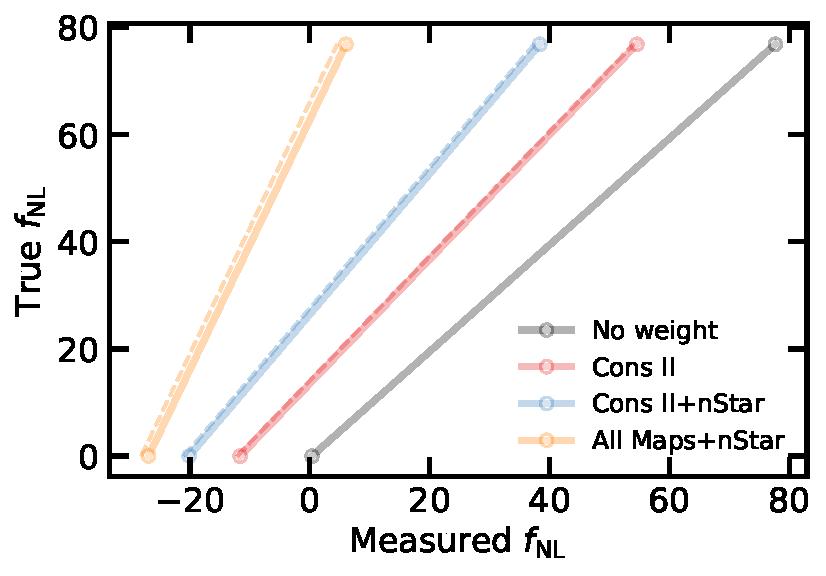
\includegraphics[width=0.45\textwidth]{figures/fnlbias}
\caption{True $\fnl$ vs measured $\fnl$ from mocks with (dashed) and without systematics (solid).}
\end{figure}